\documentclass[14pt]{article}

\usepackage[utf8x]{inputenc}
\usepackage[russian]{babel}
\usepackage{graphicx}
\graphicspath{{images/}}
\DeclareGraphicsExtensions{.pdf,.png,.jpg}

\usepackage{amsmath}
\usepackage{pgfplots}
\usepackage{makecell}

\usepackage{geometry} % Меняем поля страницы
\geometry{left=2cm}% левое поле
\geometry{right=1.5cm}% правое поле
\geometry{top=2cm}% верхнее поле
\geometry{bottom=2cm}% нижнее поле

\renewcommand{\theenumi}{\arabic{enumi}}
\renewcommand{\labelenumi}{\arabic{enumi}}
\renewcommand{\theenumii}{.\arabic{enumii}}
\renewcommand{\labelenumii}{\arabic{enumi}.\arabic{enumii}.}
\renewcommand{\theenumiii}{.\arabic{enumiii}}
\renewcommand{\labelenumiii}{\arabic{enumi}.\arabic{enumii}.\arabic{enumiii}.}

\begin{document}
\begin{titlepage}
	\begin{center}
		\fontsize{18pt}{20pt}\selectfont
		\textbf{Работа 3.4.5.}	
	
		\vspace{5cm}
		\fontsize{24pt}{25pt}\selectfont
		Петля гистерезиса (динамический метод)
	\end{center}
	\begin{flushright}
		\fontsize{18pt}{20pt}\selectfont
		\vspace{14cm}
		\hspace{-3cm}
		\textit{Корнеев Е.С.}
	\end{flushright}		
\end{titlepage}

\begin{center}
	\fontsize{16pt}{18pt}\selectfont
	Петля гистерезиса (динамический метод)
\end{center}


\fontsize{14pt}{16pt}\selectfont
\vspace{1cm}
\textbf{Цель работы:} изучение петель гистерезиса ферромагнитных материалов с помощью осциллографа.

\vspace{0.5cm}
\textbf{Оборудование:} автотрансформатор, понижающий трансформатор, интегрирующая цепочка, амперметр, вольтметр, электронный осциллограф, делитель напряжения, тороидальные образцы с двумя обмотками. 

\vspace{1cm}
Ферромагнитные материалы часто применяются в трансформаторах, дросселях, машинах переменного тока, то есть в устройствах, где они подвергаются периодическому перемагничиванию. Изучение магнитных характеристик ферромагнетиков в переменных полях представляет позтому большой практический интерес. Основные характеристики ферромагнетиков - их коэрцитивная сила, магнитная проницаемость, мощность, рассеиваемая в виде тепла при перемагничивании, и т. д. - зависят от частоты перемагничивающего поля. В настоящей работе кривые гистерезиса ферромагнитных материалов изучаются в поле частоты 50 Гц с помощью электронного осциллографа.


\textbf{Измерение магнитной индукции в образцах.} Магнитную индукцию удобно определять с помощью ЭДС, возникающей при изменении магнитного потока Ф в катушке, намотанной на образец:
\begin{equation}
\varepsilon = -\frac{d\Phi}{dt}
\end{equation}
Пусть катушка плотно охватывает образец, и индукция $B$ в образце однородна. В этом случае
\begin{equation}
\Phi = BSN,
\end{equation}
где $N$ - число витков в измерительной катушке, а $S$ - площадь витка. Подставляя это значение $\Phi$ в формулу (1), после интегрирования
найдём
\begin{equation}
|B| = \frac{1}{SN}\int \varepsilon dt
\end{equation}
Таким образом, для определения $B$ нужно проинтегрировать сигнал, наведённый меняющимся магнитным полем на измерительную катушку, намотанную на образец.

\begin{figure}[h!]
	\center{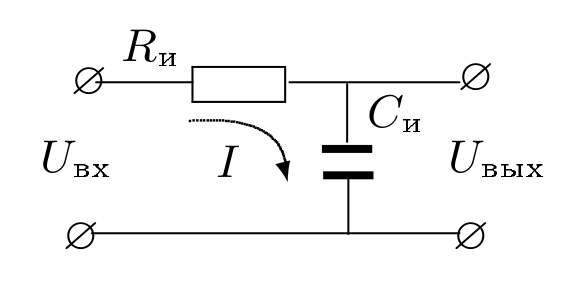
\includegraphics[width = 10cm]{1}}
	\caption{Интегрирующая $RC$-цепочка}
	\label{fig:image}
\end{figure}

Для интегрирования сигнала применяют разного рода интегрируюшие схемы. Простейшая из них состоит из соединённых последовательно резистора $R$ и конденсатора $C$ (рис. 1) и выполняет своё назначение,если сопротивление $R$ резистора заметно превышает сопротивление конденсатора (если выходной сигнал много меньше входного: 
$U_{\text{вых}} \ll U_{\text{вх}}$).

В самом деле, при при выполнении этого условия ток в цепи пропорционален входному напряжению: $I \approx U_{\text{вх}}/R$, а напряжение на ёмкости $C$
\begin{equation}
U_{\text{вых}} = \frac{q}{C} = \frac{1}{C}\int Idt \approx \frac{1}{RC}\int U_{\text{вх}}dt
\end{equation}
Этот вывод тем ближе к истине, чем больше постоянная времени $\tau = RC$ превосходит характерное время процесса (например, его период). Для синусоидальных напряжений
\begin{equation}
U_{\text{вых}} = \frac{U_{\text{вх}}}{RC\Omega}
\end{equation}
где $\Omega$ - частота сигнала.

Обозначив параметры интегрируюшей ячейки через $R_{\text{и}}$ и $C_{\text{и}}$, выразим индукцию $B$ с помошью формул (З) и (4) через $U_{\text{вых}}$ - напряжение
на ёмкости интегрируюшей ячейки:
\begin{equation}
|B| = \frac{1}{SN}\int 	\varepsilon dt = \frac{1}{SN}\int U_{\text{вх}} dt = \frac{R_{\text{и}}C_{\text{и}}}{SN}U_{\text{вых}}
\end{equation}

\textbf{Экспериментальная установка.} Схема установки изображена на рис. 2. Напряжение сети (220 В, 50 ГЦ) с помошью регулировочного автотрансформатора $\text{Ат}$ через разделительный понижающий трансформатор $\text{Тр}$ подаётся на намагничиваюшую обмотку $N_0$ исследуемого образца.

Действующее значение переменного тока в обмотке $N_0$ измеряется амперметром А. Последовательно с амперметром включено сопротивление $R_0$, напряжение с которого подаётся на вход $X$ электронного осциллографа (ЭО). Это напряжение пропорционально току в обмотке $N_0$, а следовательно, и напряжённости $H$ магнитного поля в образце.

Для измерения магнитной индукции $B$ с измерительной обмотки $N$ на вход $RC$-цепочки подаётся напряжение $U_\text{и}$ ($U_\text{вх}$), пропорциональное согласно (6) производной $\dot{B}$, а с интегрируюшей ёмкости $C_\text{и}$ снимается напряжение $U_C$ ($U_\text{вых}$), пропорциональное величине $B$, и подаётся на вход $Y$ осциллографа.

Замкнутая кривая, возникающая на экране, воспроизводит в некотором масштабе (различном для осей $X$ и $Y$) петлю гистерезиса. Чтобы придать этой кривой количественный смысл, необходимо установить масштабы изображения, т. е. провести калибровку каналов $X$ и $Y$ ЭО. Для этого, во-первых, надо узнать, каким напряжениям (или токам)
соответствуют амплитуды сигналов, видимых на экране, и, во-вторых, каким значениям $B$ и $H$ соответствуют эти напряжения (или токи).

\textbf{Измерение напряжения с помощью осциллографа.} Исследуемый сигнал подаётся на ВХОД $X$; величина сигнала характеризуется длиной $2x$ горизонтальной черты, наблюдаемой на экране ($x$ - отклонение от нуля - амплитуда сигнала).

Если известна чувствительность усилителя $K_x$ в вольтах на деление шкалы экрана, то удвоенная амплитуда напряжения определяется произведением
$$
	2U_{x,0} = 2x\cdot K_x
$$
Напряжение, подаваемое на ось $Y$, измеряется аналогично:
$$
	2U_{y,0} = 2y\cdot K_y
$$
где $y$ - отклонение от нуля в делениях шкалы, $K_y$ - чувствительность усилителя в В/дел.

Наличие в схеме амперметра и вольтметра позволяет провести калибровку усилителей ЭО, т.е. проверить значения коэффициентов $K_x$ и $K_y$, (или определить их, если ручки плавной регулировки усиления при измерениях не были установлены на максимум).

\textbf{Калибровка горизонтальной оси ЭО} проводится при закороченной обмотке $N_0$. Эта обмотка с помещённым в неё ферромагнитным образцом является нелинейным элементом, так что ток в ней не имеет синусоидальной формы, и это не позволяет связать амплитуду тока с показаниями амперметра.

При закороченной обмотке $N_0$ амперметр А измеряет эффективное значение синусоидального тока $I_\text{эфф}$, текущего через известное сопротивление $R_0$. Сигнал с этого сопротивления подаётся на вход $X$ ЭО. Измерив $2x$ - длину горизонтальной прямой на экране, можно рассчитать $m_x$ - чувствительность канала $X$:
\begin{equation}
m_x = \frac{2R_0\sqrt{2}I_\text{эфф}}{2x} \frac{\text{В}}{\text{Дел}}
\end{equation}

\textbf{Калибровка вертикальной оси} проводится с помощью сигнала, снимаемого через делитель напряжения с обмотки 12,6 В понижающего трансформатора (рис. 2). Вольтметр $V$ измеряет напряжение $U_\text{эфф}$ на обмотке. Часть этого напряжения снимается с делителя с коэффициентом деления $K$ и подаётся на вход $Y$ ЭО (вместо напряжения ПО на рис. 2).

\begin{figure}[h!]
	\center{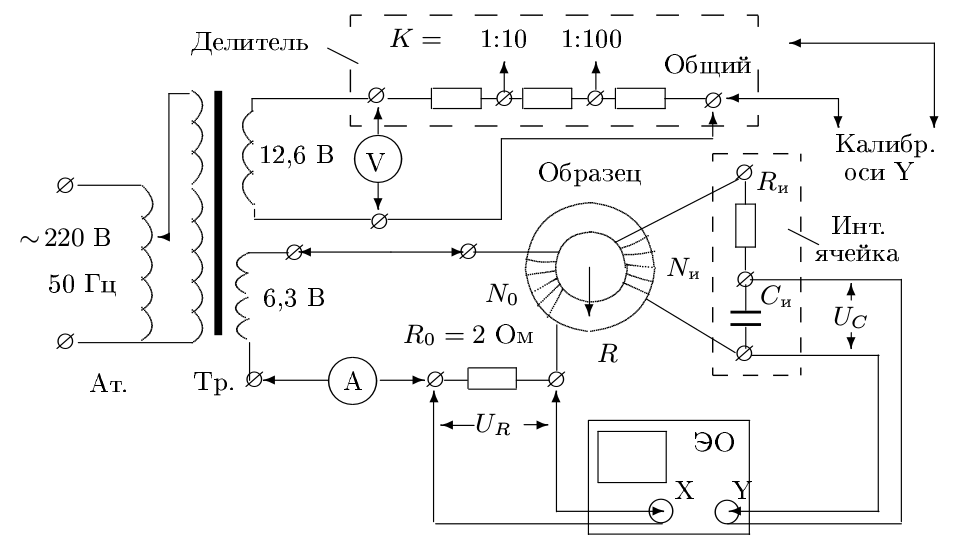
\includegraphics[width = 16cm]{2}}
	\caption{Схема установки}
	\label{fig:image}
\end{figure}

Измерив $2y$ - длину вертикальной прямой на экране, можно рассчитать чувствительность канала $Y$:
\begin{equation}
m_y = \frac{2\sqrt{2}KU_\text{эфф}}{2y} \frac{\text{В}}{\text{Дел}}
\end{equation}

При калибровке канала $Y$ тороид должен быть отключён, так как несинусоидальный ток нагрузки в первичной обмотке $N_0$ тороида приводит к искажению формы кривой напряжения и на обмотке трансформатора, питающей делитель.

Калибровку осей осциллографа можно использовать для построения кривой гистерезиса в координатах $B$ и $H$. Значения $H$ рассчитываются по теореме о циркуляции, значения $B$ - по формуле (6).

\textbf{Постоянную времени $RC$-цепочки} можно определить экспериментально. С обмотки 6,3 В на вход интегрирующей цепочки подаётся синусоидальное напряжение $U_\text{вх}$. На вход $Y$ осциллографа поочерёдно подаются сигналы со входа ($U_\text{вх}$) и выхода ($U_\text{вых} = U_C$) $RC$-цепочки. Измерив амплитуды этих сигналов с помощью осциллографа, можно рассчитать постоянную времени $\tau = RC$. Как следует из формулы (5),
\begin{equation}
RC = \frac{U_\text{вх}}{RU_\text{вых}}
\end{equation}

\newpage

\textbf{Ход работы.}

\vspace{1cm}
0. Соберем схему согласно рис. 2 и подготовим приборы к работе. Сведем в таблицу характеристики устновки.

\begin{center}
\begin{tabular}{|c|c|c|c|c|c|c|c|c|c|c|c|}
\hline
						&	Феррит	&	Пермаллой	&	Кремнистое железо	\\
\hline
$N_0$, витков			&	35		&	40			&	35					\\
\hline
$N_\text{и}$, витков	&	400		&	200 		&	350					\\
\hline
$S$, см$^2$				&	3.0		&	3.8			&	1.2					\\
\hline
$2\pi R$, см			&	25		&	24			&	10					\\
\hline
\end{tabular}
\end{center}

1. Снимем зачения, соответсвтующие вершинам петель гистерезиса, подбирая ток питания таким, чтобы предельная петля гистерезиса занимала большую часть экрана. 

\begin{center}
\begin{tabular}{|c|c|c|c|c|c|c|c|c|c|c|c|c|c|}
\hline
\multicolumn{3}{|c}{Феррит}			&	\multicolumn{3}{|c}{Пермаллой}			&	\multicolumn{3}{|c|}{\makecell{Кремнистое \\ железо}}	\\
\hline
$I$, А	&	$x$, дел&	$y$, дел	&	$I$, А	&	$x$, дел	&	$y$, дел	&	$I$, А	&	$x$, дел	&	$y$, дел				\\
\hline				
0.054	&	1.2		&	1.0			&	0.065	&	1.2			&	0.4			&	0.167	&	1.0			&	1.0						\\
\hline
0.097	&	2.0		&	1.6			&	0.088	&	1.8			&	0.8			&	0.241	&	1.6			&	1.4						\\
\hline
0.156	&	2.8		&	2.0			&	0.100	&	2.0			&	1.0			&	0.321	&	2.4			&	1.6						\\
\hline
0.169	&	3.2		&	2.2			&	0.114	&	2.4			&	1.2			&	0.412	&	3.0			&	1.8						\\
\hline
0.201	&	3.6		&	2.4			&	0.132	&	3.2			&	1.8			&	0.460	&	4.0			&	2.0						\\
\hline
0.223	&	4.2		&	2.6			&			&				&				&			&				&							\\
\hline
0.240	&	5.0		&	2.8			&			&				&				&			&				&							\\
\hline
\end{tabular}
\end{center}

\vspace{0.5cm}
Примем погрешность $\sigma_x = 0.1$ дел, так как на единицу шкалы на экране осциллографа приходилось малых 5 делений. Аналогично, $\sigma_y = 0.1$ дел. Погрешность 
же $\sigma_I$ будет равна 1 мА. 

\newpage
Построим соответствующие кривые намагничивания.

\begin{tikzpicture}
\begin{axis}[
	title  = {Феррит},
	height = 8cm,
	width  = 15cm,
	every axis y label/.style={at = {(ticklabel cs: 0.5)}, rotate = 90, anchor = near ticklabel},
	xlabel = {$x$, дел},
	ylabel = {$y$, дел},
	grid   = major,
	xmin = 0,
	ymin = 0,
]

\addplot+[
	only marks,
	error bars/.cd, 
	y dir = both, y explicit,
	x dir = both, x explicit
	]
coordinates{
	(1.0, 0.8)	+-	(0.1, 0.1)
	(2.0, 1.6)	+-	(0.1, 0.1)
	(2.8, 1.8)	+-	(0.1, 0.1)
	(3.2, 2.2)	+-	(0.1, 0.1)
	(3.6, 2.4)	+-	(0.1, 0.1)
	(4.2, 2.6)	+-	(0.1, 0.1)
	(5.0, 2.8)	+-	(0.1, 0.1)
};

\addplot+[
	mark  = none,
	smooth,
	color = blue
	]
coordinates{
	(  0,   0)
	(1.0, 0.9)
	(2.0, 1.55)
	(2.8, 2.0)
	(3.2, 2.2)
	(3.6, 2.4)
	(4.2, 2.6)
	(5.0, 2.8)
};

\end{axis}
\end{tikzpicture}

\begin{tikzpicture}
\begin{axis}[
	title  = {Пермаллой},
	height = 8cm,
	width  = 15cm,
	every axis y label/.style={at = {(ticklabel cs: 0.5)}, rotate = 90, anchor = near ticklabel},
	xlabel = {$x$, дел},
	ylabel = {$y$, дел},
	grid   = major,
	xmin = 0,
	ymin = 0,
]

\addplot+[
	only marks,
	error bars/.cd, 
	y dir = both, y explicit,
	x dir = both, x explicit
	]
coordinates{
	(1.2, 0.4)	+-	(0.1, 0.1)
	(1.8, 0.8)	+-	(0.1, 0.1)
	(2.0, 1.0)	+-	(0.1, 0.1)
	(2.4, 1.2)	+-	(0.1, 0.1)
	(3.2, 1.8)	+-	(0.1, 0.1)
};

\addplot+[
	mark  = none,
	smooth,
	color = blue
	]
coordinates{
	(  0,   0)
	(1.2, 0.45)
	(1.8, 0.78)
	(2.0, 0.93)
	(2.4, 1.2)
	(3.2, 1.8)
};

\end{axis}
\end{tikzpicture}

\begin{tikzpicture}
\begin{axis}[
	title  = {Кремнистое железо},
	height = 8cm,
	width  = 15cm,
	every axis y label/.style={at = {(ticklabel cs: 0.5)}, rotate = 90, anchor = near ticklabel},
	xlabel = {$x$, дел},
	ylabel = {$y$, дел},
	grid   = major,
	xmin = 0,
	ymin = 0,
]

\addplot+[
	only marks,
	error bars/.cd, 
	y dir = both, y explicit,
	x dir = both, x explicit
	]
coordinates{
	(1.0, 1.0)	+-	(0.1, 0.1)
	(1.6, 1.4)	+-	(0.1, 0.1)
	(2.4, 1.6)	+-	(0.1, 0.1)
	(3.0, 1.8)	+-	(0.1, 0.1)
	(4.0, 2.0)	+-	(0.1, 0.1)
};

\addplot+[
	mark  = none,
	smooth,
	color = blue
	]
coordinates{
	(  0,   0)
	(1.0, 1.0)
	(1.6, 1.4)
	(2.4, 1.7)
	(3.0, 1.85)
	(4.0, 2.0)
};

\end{axis}
\end{tikzpicture}

\vspace{1cm}
При измерениях использовались следующие диапазоны, а также были получены следующие значения $2x$ и $2y$:

\begin{center}
\begin{tabular}{|c|c|c|c|c|c|c|c|c|c|c|c|c|c|c|c|c|c|}
\hline
						&	Феррит		&	Пермаллой	&	Кремнистое железо	\\
\hline
$K_x$, мВ/дел			&	20			&	20			&	50					\\
\hline
$K_y$, мВ/дел			&	20			&	100			&	100					\\
\hline
$2x$, дел				&	1.8			&	1.8			&	0.6					\\
\hline
$2y$, дел				&	1.8			&	3.2			&	1.4					\\
\hline
$m_x$, мВ/дел			&	22			&	18			&	48					\\
\hline
$m_y$, мВ/дел			&	23			&	96			&	95					\\
\hline
$H$, А/м дел			&	34			&	22.0		&	160					\\
\hline
$B$, Тл/дел				&	0.19		&	0.91		&	0.70				\\
\hline
\end{tabular}
\end{center}

\vspace{1cm}
Определим значения $\sigma_H$ и $\sigma_B$. Считая $H = f(x, K_x)$, $B = f(y, K_y)$ (?), по формуле
$$
	\sigma = \sqrt{\sum_{k = 1}^n \left(\frac{\partial f}{\partial x_k}\sigma_{x_k}\right)^2}
$$
найдем значения погрешностей:
\begin{center}
\begin{tabular}{|c|c|c|c|c|c|c|c|c|}
\hline
					&	$\sigma_H$, А/м дел		&	$\sigma_B$, Тл/дел	\\
\hline
Феррит				&	2						&	0.01				\\
\hline
Пермаллой			&	1						&	0.03				\\
\hline
Кремнистое железо	&	10						&	0.04				\\
\hline
\end{tabular}
\end{center}


\vspace{1cm}
Теперь из графиков можно определить значения $\mu$ и $H_c$ и $B_s$

\begin{center}
\begin{tabular}{|c|c|c|c|c|c|c|c|c|c|c|c|}
\hline
			&	Феррит	&	Пермаллой	&	Кремнистое железо	\\
\hline
$\mu$		&	3200	&	13200		&	3500				\\
\hline
$H_c$,А/м	&	62		&	40			&	96					\\
\hline
$B_s$,Тл	&	0.40	&	2.7			&	2.1					\\
\hline
\end{tabular}
\end{center}

Им соответствуют погрешности

\begin{center}
\begin{tabular}{|c|c|c|c|c|c|c|c|c|c|c|c|}
\hline
				&	Феррит	&	Пермаллой	&	Кремнистое железо	\\
\hline
$\sigma_\mu$	&	500 	&	2400		&	600					\\
\hline
$H_c$,А/м		&	6		&	4			&	9					\\
\hline
$B_s$,Тл		&	0.05	&	0.3			&	0.2					\\
\hline
\end{tabular}
\end{center}

Погрешность $\sigma_\mu$ найдем по формуле
$$
	\sigma_\mu = \sqrt{\sigma^2_\text{случ} + \sigma^2_\text{приб}},
$$
где $\sigma^2_\text{случ}$ определим по МНК. 
Погрешности $\sigma_{H_c}$ и $\sigma_{B_s}$ найдем, считая $H_c = f(\Delta H_c, x)$, $B_s = f(\Delta B_s, y)$.

\vspace{1cm}
Определим значение $\tau = RC$ экспериментально по формуле
$$
	\tau = \frac{U_\text{вх}}{\Omega U_\text{вых}} = \frac{6.3 \text{В}}{50\cdot2\pi~c^{-1} \cdot 0.049 \text{В}} = 0.41~c
$$
Видно, что полученное значение почти не отличается от "номинального":
$$
	\tau = RC = 20\cdot10^{3}\text{Ом} \cdot 20\cdot10^{-6}\text{Ф} = 0.4~c
$$

На выходе для RC - 0.05 В примерно

\newpage
Таким образом, в данной лабораторной работе мы изучили поведение некоторых материалов (а именно феррита, кремнистого железа и пермаллоя) в переменном магнитном поле, а также определили некоторые характеристики этих веществ. 








\end{document}